\section{Introduction}
\label{sec:intro}

A number of distributed services and applications need to measure
Internet paths to maintain an up-to-date view of the underlying
infrastructure~\cite{duffield06binary,
dhamdhere07netdiagnoser,kompella07blackholes,
bassett12lifeguard,akamai,skitter}. All these systems use some version
of traceroute to repeatedly measure a large number of Internet paths.
Traceroute sends probes to every hop between a source and a destination,
so the measurement of a single path often requires tens of probes and
takes some seconds~\cite{veitch09balancer}. The number of probes required
to measure a path is even larger if one wants to measure all paths
between a source and a destination when routers perform load
balancing~\cite{veitch09balancer}. For example, discovering a
(multi)path with Paris traceroute, which is a traceroute version that
discovers all paths under load balancing, requires hundreds of probes
and takes tens of seconds~\cite{veitch09balancer}.\footnotemark{}
Because measuring each path takes time, a source cannot measure paths
frequently and as a result it may miss path changes. For instance,
topology mapping systems can take from several minutes to a few days to
measure all required paths~\cite{cunha11fastmapping, sherwood08discarte,
skitter}.  In between measurements, paths may be outdated or
inconsistent.

\footnotetext{
% Given the
% prevalence of load balancing in the Internet~\cite{augustin07},
It is essential to accurately measure paths under load balancing to avoid
traceroute errors and misinterpretation of path
changes~\cite{cunha11fastmapping}.}

Our previous work showed that Internet paths being mostly stable,
measuring all paths at the same frequency wastes probes in paths that
are not changing~\cite{cunha11dtrack}. We developed \dtrack{}, a system
that optimizes probing to track Internet path
changes~\cite{cunha11dtrack}.  \dtrack{} splits the task of tracking
paths into two sub-tasks.  \textit{Path change detection} sends a single
probe per path at any given time, probing more frequently paths that are
more likely to change. \textit{Path remapping} responds to a path change detection
by immediately sending probes to discover all interfaces of the new multipath.
Although \dtrack{} detects twice as many path changes
as traditional probing~\cite{cunha11dtrack}, remapping a path remains
costly.  \dtrack{} simply runs Paris traceroute to remap the entire
end-to-end path. Such complete remapping ensures the accuracy of
inferred paths, but incurs a large probing overhead.

In this paper, we show that complete remapping wastes probes because
most path changes are localized in a few (consecutive) hops of a path
(\secstr~\ref{sec:char}). We build on this observation to develop a more
efficient remapping method for \dtrack{} (\secstr~\ref{sec:remap}).
Given knowledge of the path before the change and the hop where the
change was detected, we first send probes to precisely locate the change and then
just remap the (generally few) hops that have changed. We call this
method \textit{local remapping} as opposed to the complete remapping
originally implemented in \dtrack{}. Local remapping still uses Paris
traceroute's multipath detection algorithm~\cite{veitch09balancer} for
discovering all interfaces at a given hop to guarantee accuracy, but we
no longer have to remap every single hop of the path.

Our evaluation via trace-driven simulations shows that local remapping
reduces the remapping probing cost of 88\% of path changes in our dataset by
more than half, and reduces overall cost by 73\% (\secstr~\ref{sec:sim}).
Local remapping has two  limitations: (i) it may only remap part of the
change when paths change in multiple locations; and (ii)  it does not
work when a path change reorders the interfaces of the path.  We show
that local remapping accurately remaps all changes in a path for 87\%
of path changes and that less than 1\% of path changes reorder hops
(\secstr~\ref{sec:sim}).  We develop a new version of \dtrack{} with
local remapping.  Our evaluation in a PlanetLab deployment shows that
local remapping inferences are identical to those obtained with complete
remapping for 92\% of path changes (\secstr~\ref{sec:deploy}). Yet,
local remapping reduces overall probing cost by 75\% when compared with
complete remapping.
\pagebreak

An early version of this work appeared (in Portuguese) at the Brazilian
Computer Networks and Distributed Systems Symposium~\cite{cunha13remap}.
Here we improve the path change remapping formalism and give an
evaluation with larger data sets.

% If we use the probes we save by using local remapping for detection,
% our new version of \dtrack{} can track \ed{XXX} more path changes than
% the original \dtrack{} with end-to-end remapping and \ed{XXX} more
% changes than traditional probing.

%
%Reducing remapping costs increases the number of probes available for
%topology mapping.  We can use the extra probes to monitor more paths and
%improve network coverage, or we can increase probing frequency and
%improve routing change tracking.  \rmprt{} is another step toward
%building more complete and consistent Internet maps.

%Internet failure identification systems usually require information
%about network routes~\cite{duffield06binary, dhamdhere07netdiagnoser,
%kompella07blackholes, bassett12lifeguard}.  Similarly, content
%distribution networks measure Internet routes to choose the ``best''
%server to answer a request~\cite{akamai}.  These and other systems
%measure routes frequently in an attempt to track routing changes as they
%happen.
%
%Internet route measurements are usually performed with
%traceroute~\cite{veitch09balancer, spring02rocketfuel,
%madhyastha06iplane}, which sends probes to identify a sequence of
%interfaces between a source and a destination.  The bandwidth available
%to send probes is finite.  Route measurements for topology mapping
%require a large number of probes and can take from several minutes to a
%few days~\cite{cunha11fastmapping, sherwood08discarte, skitter}.  It is
%impossible to measure routes frequently enough to detect all routing
%changes without overloading the network.  Thus, Internet topology maps
%may be outdated, or inconsistent as routing changes may occur during the
%measurement process.
%
%Our \dtrack{} system tracks Internet routing changes to keep Internet
%topology maps more up-to-date~\cite{cunha11dtrack}.  \dtrack{} separates
%the tasks of detecting and remapping routing changes.  To detect
%changes, \dtrack{} uses a lightweight probing process that combines two
%main ideas: (1) redirect probes from stable paths, where routing changes
%are unlikely, to unstable paths, where routing changes are more likely;
%and (2) spreading probes uniformly over the network and over time to
%reduce redundant probes.  \dtrack{} keeps a database with the previous
%route observed on each monitored path.  \dtrack{} sends a probe to a hop
%in the path and compares the IP address in the reply with the IP address
%in the previous route.  If the probe reply is incompatible with the
%previous route, e.g., the IP address in the probe reply is not in the
%previous route, a change is detected and the remapping process is
%triggered.
%
%To remap changes, \dtrack{} uses Paris
%traceroute~\cite{veitch09balancer} to measure the current route.  Paris
%traceroute is an improved version of traceroute that identifies routers
%that perform load balancing.  \dtrack{} uses Paris traceroute because it
%is impossible to differentiate routing changes from load balancing
%otherwise~\cite{cunha11fastmapping}.  Currently, \dtrack{} remaps the
%whole path using Paris traceroute.  This approach guarantees correct
%remapping of the current route, but wastes probes as most routing
%changes involve few hops (\secstr~\ref{sec:char}).  In particular, this
%approach ignores two pieces of information available when the remapping
%process begins: the previous route and the hop where the change was
%detected.
%
%In this paper we propose \rmprt{}, a new tool to reduce the cost of
%remapping Internet routing changes (\secstr~\ref{sec:remap}).  Given the
%previous route observed before the change and a hop where a change was
%detected, \rmprt{} strategically sends probes to locate the change and
%locally remap it rather than waste probes on an unnecessary complete
%remapping.
%
%Our evaluation via trace-driven simulations shows that \rmprt{} reduces
%by half the remapping cost of 88\% of routing changes in our dataset
%(\secstr~\ref{sec:sim}).  Remap cost reduction is even larger for routes
%traversing routers that perform load balancing.  RemapRoute's
%optimizations do not work if a previous route measurement is unavailable
%or if a routing change reorders hops (0.9\%), but is otherwise
%statistically equivalent to Paris traceroute (\secstr~\ref{sec:sim}).
%Our evaluation of \rmprt{} in a real deployment confirms our simulation
%results and demonstrates \rmprt{}'s accuracy (\secstr~\ref{sec:deploy}).
%We make the following contributions:
%
%% FIGS 1--3 FROM SEC. 3
%\begin{figure*}[t]
%\begin{minipage}{0.33\textwidth}
%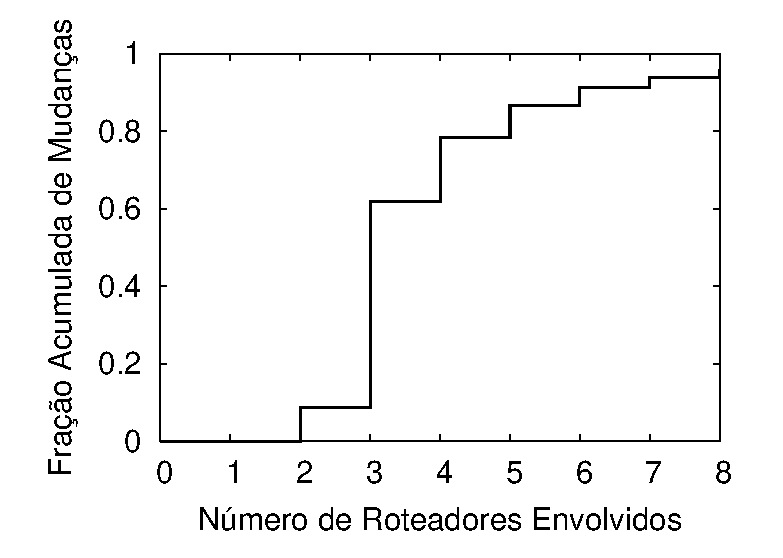
\includegraphics[width=1.05\textwidth]{figs/nrouters.eps}
%\caption{Distribution of the number of hops involved in path changes.}
%\label{fig:char.nrouters}
%\end{minipage}
%\hfill
%\begin{minipage}{0.33\textwidth}
%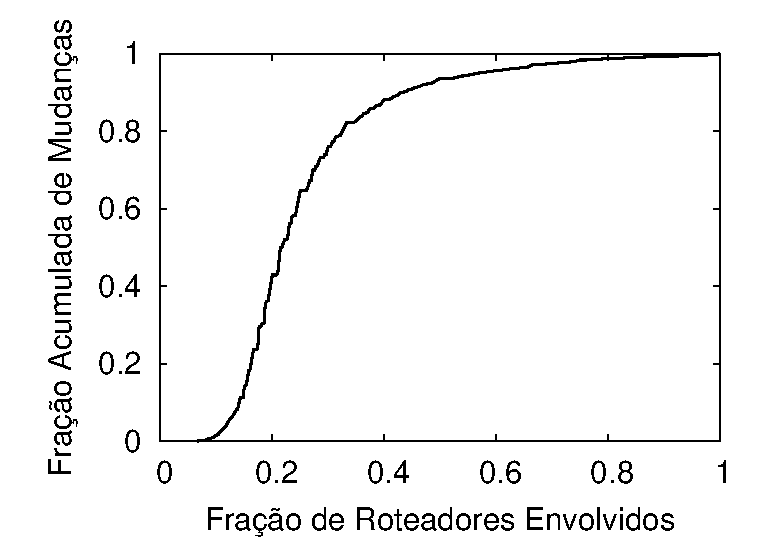
\includegraphics[width=1.05\textwidth]{figs/fracs.eps}
%\caption{Distribution of the fraction of routers involved in path changes.}
%\label{fig:char.fracs}
%\end{minipage}
%\hfill
%\begin{minipage}{0.33\textwidth}
%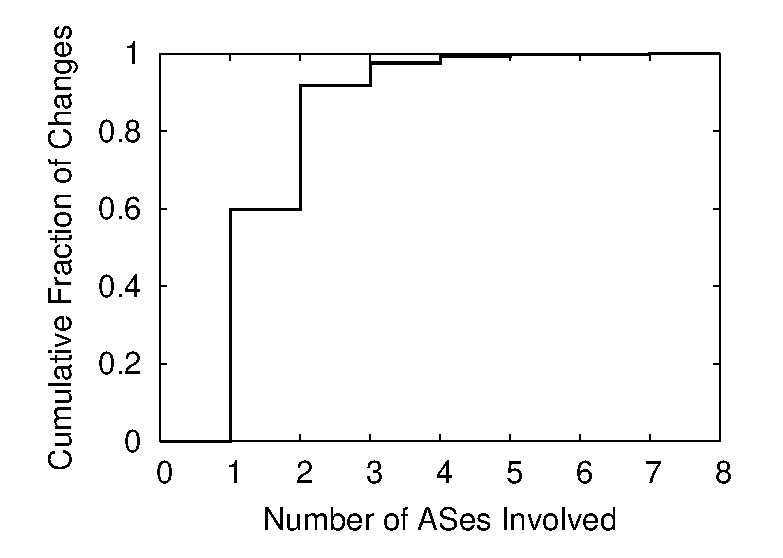
\includegraphics[width=1.05\textwidth]{figs/nasns.eps}
%\caption{Distribution of the number of ASes involved in path changes.}
%\label{fig:char.nasns}
%\end{minipage}
%\end{figure*}
%
%\begin{itemize}
%%
%\item We characterize Internet routing changes and show that they
%usually involve few hops (\secstr~\ref{sec:char});
%%
%\item We propose methods to locate and remap path changes that reduce
%wasted probes (\secstr~\ref{sec:remap});
%%
%\item We show the efficacy of our tool with trace-driven simulations and
%in a real deployment (\secstrs~\ref{sec:sim} and~\ref{sec:deploy}).
%%
%\end{itemize}
%
%Reducing remapping costs increases the number of probes available for
%topology mapping.  We can use the extra probes to monitor more paths and
%improve network coverage, or we can increase probing frequency and
%improve routing change tracking.  \rmprt{} is another step toward
%building more complete and consistent Internet maps.


